\addtocontents{toc}{\protect\newpage}
\chapter{Backends}
\label{chapter:backend}

\chapterprecishere{You are responsible for the predictable consequences of your actions.\par\raggedleft--- \textup{Noam Chomsky}}
\chapterhung

\index{backend|boldindex}

System administrators are rarely confronted with the developer's frontends.
They are concerned about making applications in the system work together as a whole.
In this section we deal with modular and programmable backends.
We explore extensions of \elektra{Spec} for these needs, answering the research question:
\rqBackend*

Only a hand-full factors determine how well an application is integrated into its system, for example:
logging, available external interfaces, look\&feel of the user interface, and user interaction (such as shortcuts and menus).
In modern applications these aspects are configurable.
We attempt to exploit already present configuration access points to make the system feel as if it was made from one piece~\cite{raab2015kps}.

Currently, such an endeavor requires a user to configure each application manually.
We have an instance of the \empha{configuration integration problem} as described in~\secref{introduction-configuration-integration}.
In this chapter, we mitigate the configuration integration problem by introducing a system-wide, programmable \empha{key database}.
The key database can be accessed by any of the frontends described earlier.

In~\secref{configuration-abstractions}, we describe how abstractions help in solving the configuration integration problem.
We describe the history of earlier failed attempts to create a universal backend and show how modularization of backends helped to overcome the challenges.
Then we elaborate on the current state of how to integrate already existing configuration files into the system-wide key database using backends.

In~\secref{backend-context-aware-lookup}, we elaborate on context-aware lookups in the key database.
We describe how layers are integrated in the backend.
We assume that applications use one of the frontends discussed in the previous chapter.

In~\secref{modular-abstractions}, we get rid of the assumption that application's source code needs to be modified and integrate already existing frontends.
We show how the key database helps us to integrate applications without compromising modularity.
We demonstrate improved modularity in the areas of suitable configuration settings and configuration validation.

In~\secref{unmodified-floss}, we elaborate on how to adapt widely used frontends.
We present a solution of how to improve context awareness of applications without any modifications in the source code.%
{\parfillskip=0pt plus .8\textwidth \emergencystretch=.5\textwidth \par}





\section{Configuration Abstractions}
\label{sec:configuration-abstractions}

In this section we describe different levels of configuration abstractions, exploring the research question:
\rqBackendDesignDecisions*

\subsection{History}

As in the frontend, also in the backend the most problematic part was too weak or wrong abstraction.
In particular, passing out internals about the backends caused many hard-to-fix problems.

In the first versions of \elektra{}, every key had a direct relation to a file in the file system.
The metadata of the key was the metadata of the file, for example, access permissions.
Soon we realized that this abstraction is poor.
Limitations of file systems directly affected \elektra{}.
For example, every persisted key in its own file needed the block size of the underlying file system.
At that time, the block size usually was 4 kilobytes, but many configuration values only have the size of a few bytes.

Out of necessity, we enabled system administrators to choose between different backends.
We implemented a Berkeley DB backend to avoid the mentioned waste of resources.
In these backends, the leaky abstractions were troublesome:
The metadata and the direct relation to files was not useful anymore.

Even more problematic was the semantics to get or set individual keys.
It was time-consuming to implement backends, which serialized configuration settings to configuration files:
It was a complicated endeavor to modify a single ^Key^ in the middle of the configuration file efficiently.
We have to check if a different process modified the file (conflict-detection), parse the file, do the necessary modifications, and write the changes back.
This implementation has to be repeated for every configuration file parser.

For \elektra{} 0.7, released on \formatdate{17}{10}{2008}, we thought of the following solution:
We wanted to use capabilities to describe what a backend is able to do.
If a backend cannot change individual keys within the file, its capabilities would say so.
The capabilities were a way to describe that backends were incompatible to some file system semantics.
Unfortunately every backend, except for file system backends, was incompatible in some way.
The capability descriptions were long and complicated.

From the user's point of view, most of the backends were not an option:
If a single application needed a specific capability, the user is already tied to the specific backend.
To defuse the situation, we introduced a way to \empha{mount} several backends into the system-wide key database.
Hence, if an application had specific requirements for the backend, we mount this particular backend.

In \elektra{} 0.8 released on \formatdate{5}{5}{2012}, we implemented a full abstraction in that frontends are no longer able to distinguish between different kinds of backends.
Backends only differ in:
\begin{itemize}
\item Their quality characteristics, such as their performance.
\item The kind of configuration settings they accept and reject.
\item Characteristics important for system administrators and legacy systems, such as the configuration file format.
\end{itemize}


This history resembles that of file systems.
Our solution is similar to what modern virtual file systems provide.
The main difference to file systems is that \elektra{}:
\begin{itemize}
\item
builds upon key-value pairs and not files, and
\item
provides configuration abstractions such as default values and transformation.
\end{itemize}





\subsection{Key Database}

Here we have a top-down discussion of the configuration abstraction included in the key database.
The \empha{key database} stores all configuration settings in configuration files.
This way, the operating system takes care of security via file system permissions~\cite{raab2016unanticipated}.

The bootstrapping (see \secref{bootstrapping}) is important to fulfill Requirement~\reqref{simple}:
\reqSimple*

It is a prerequisite to have a global view to enable sharing of configuration settings:
\reqSharing*



\subsubsection{Plugins}
\label{sec:plugins}

\newcommand{\nrplugins}{78}


The backends delegate their complete work to plugins.
We recently added many plugins to support even more functionality for configuration access.
The figure on page~\pageref{fig:plugins} shows the current state of plugins with dependences.
For some functionality, we are already aware of a saturation:
Only small details are missing.
For other functionality, such as supporting more configuration file formats and validation specifications, we currently do not see any limitation for the number of plugins that would be useful.



Implementing too many features in one plugin is problematic.
Many aspects would clutter the source code, making the plugins difficult to maintain.
To alleviate this problem, \intro{several plugins} together build up a backend.
Each plugin implements a single concrete requirement, as standard in many architectures~\cite{pinson1978unix,cardozo2016emergent}.
Hence, we ended up with the large number of \nrplugins{} plugins as shown in full-page figure on the next page.
Arrows indicate plugins that \empha[provider]{provide} some abstract functionality.
Square boxes are providers.
Names in ellipses are concrete plugins not used as provider names.
We did not include plugins without arrows.


The architecture allows plugins to have external dependences without adding the dependence to \elektra{}'s core.
Not every plugin has the burden to be portable, instead highly-optimized plugins are useful alternatives to generic plugins.
With this separation, each plugin and the core of \elektra{} stays minimal.

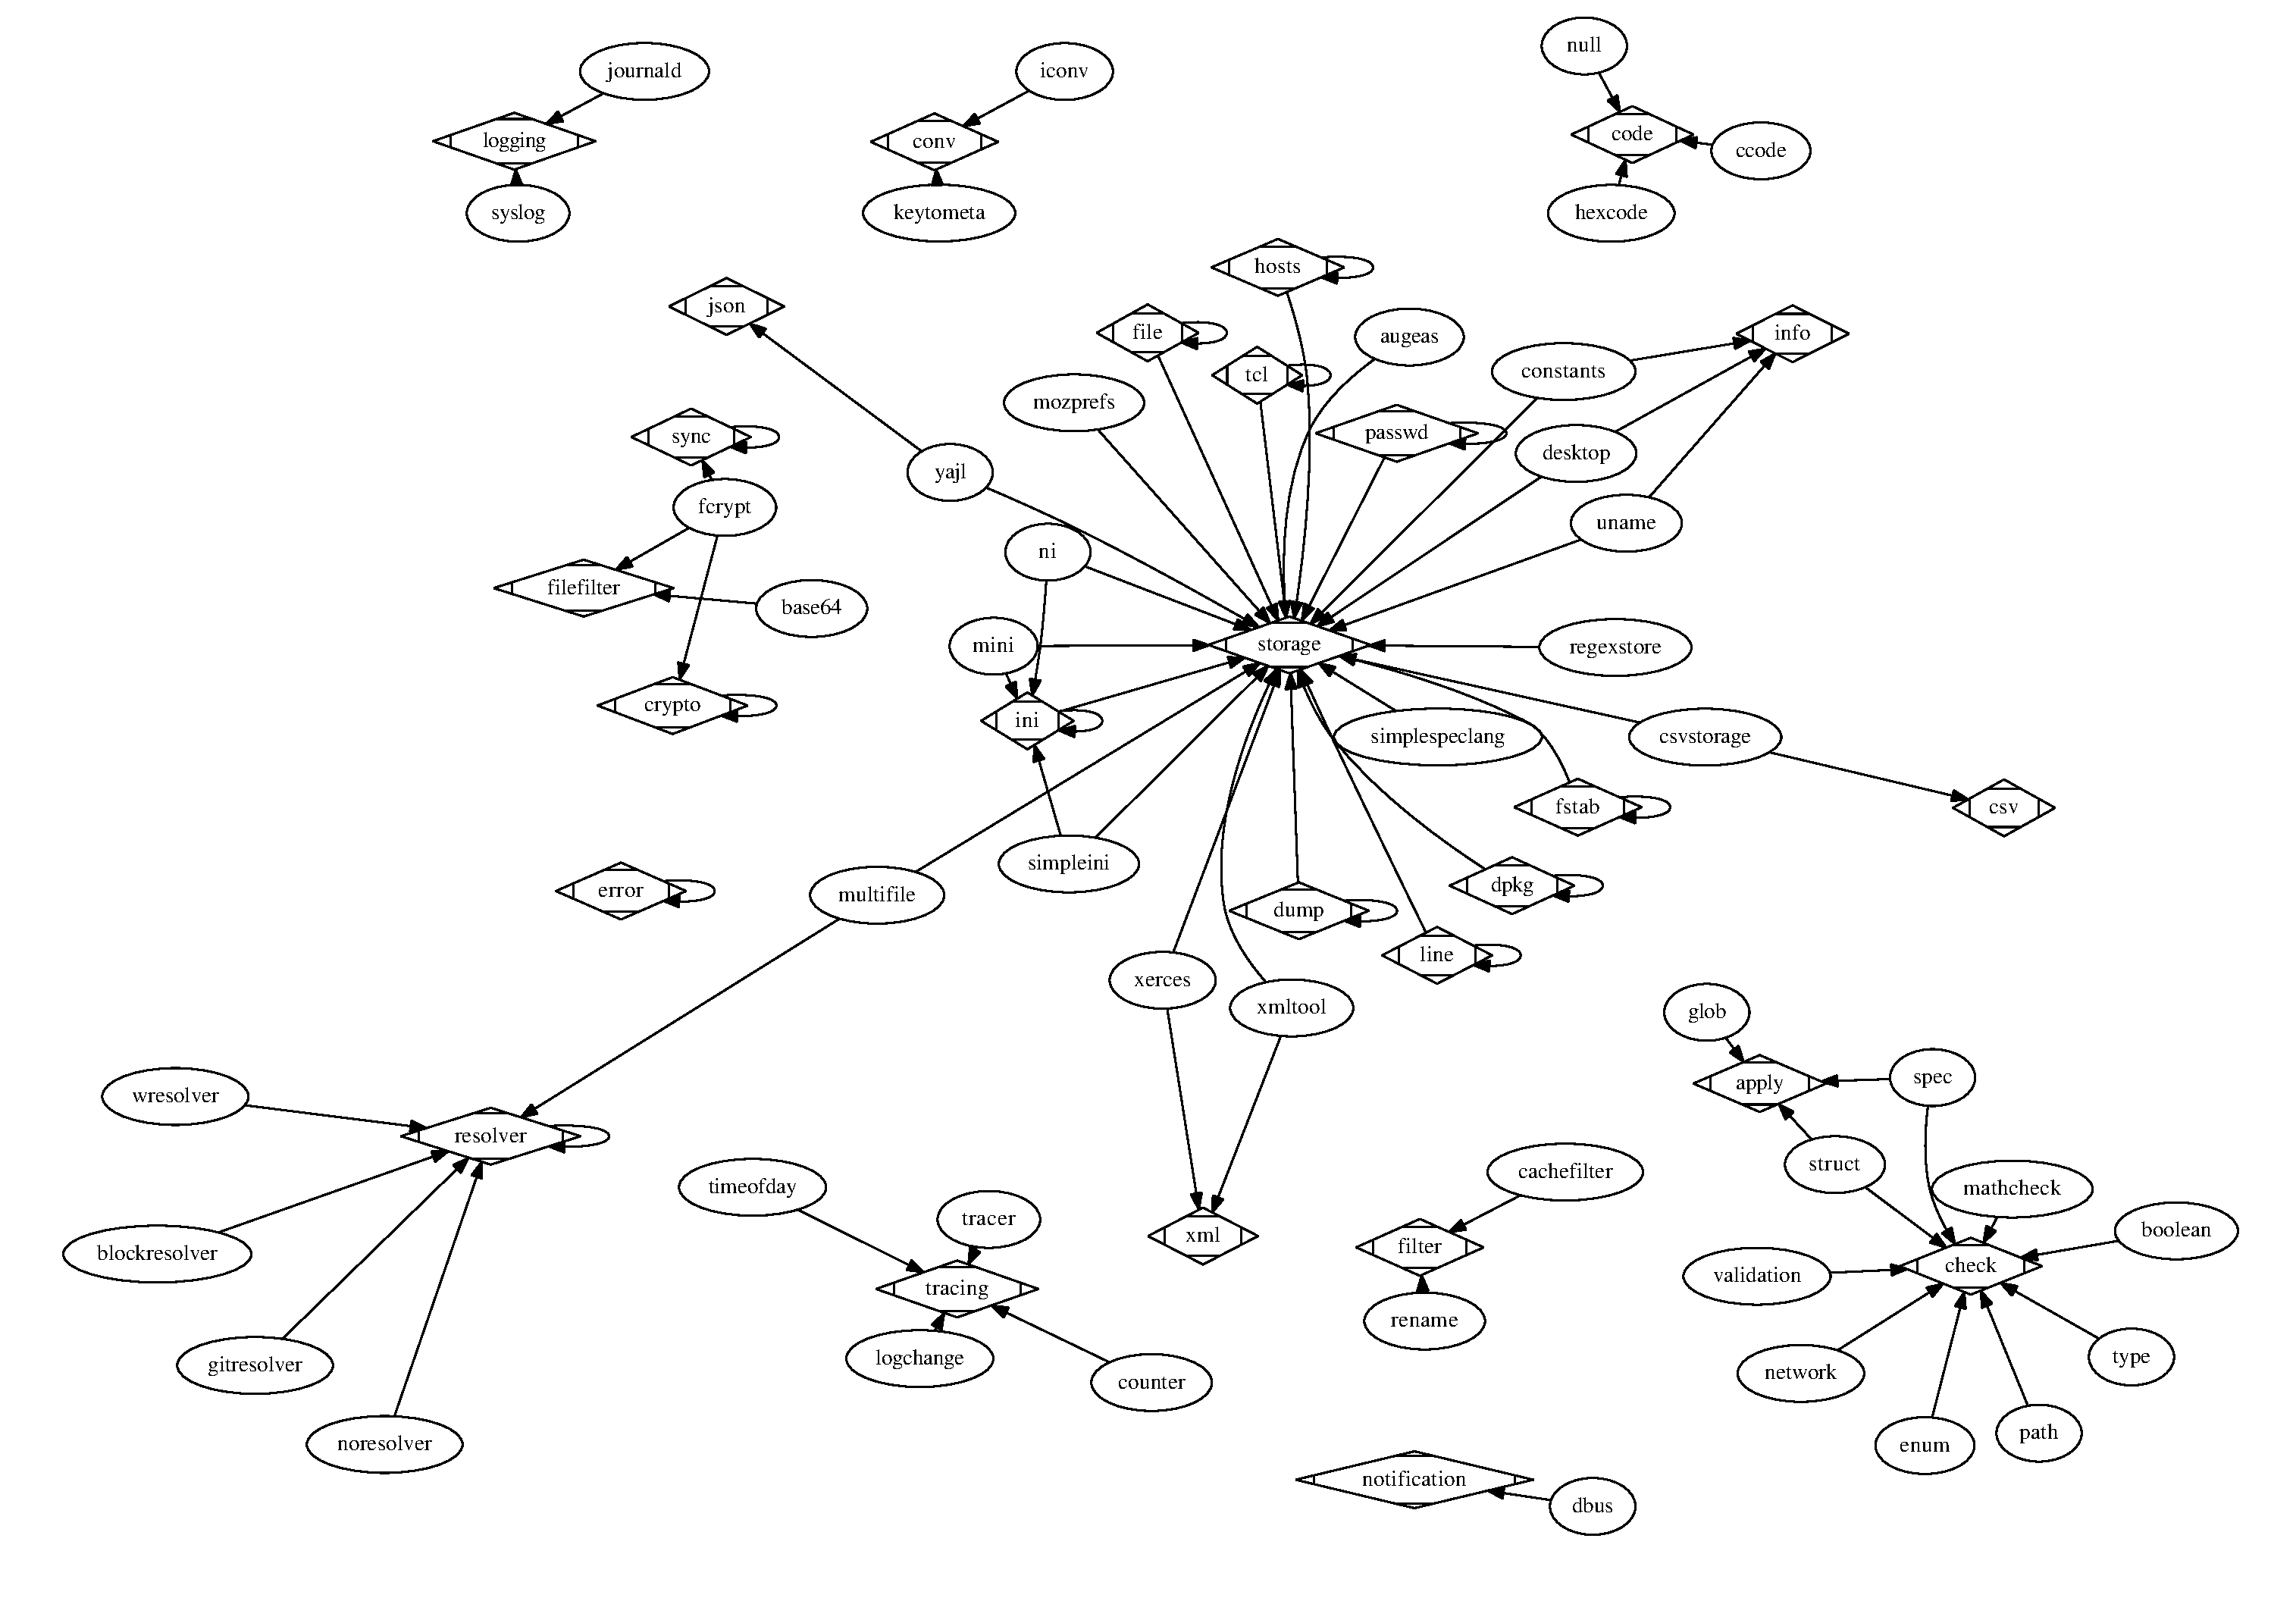
\includepdf[landscape=true,offset=15 00,addtolist={1, figure, Plugins, fig:plugins},]{figures/plugins.pdf}


\subsubsection{Storage Plugins}

Configuration file formats have countless variations in their syntax.
The repository of Augeas~\cite{lutterkort2008augeas} (that covers a small part of GNU/Linux configuration files) already contains lenses for 181 configuration file formats.
Plugins concerned with parsing and serializing configuration files are called \intro[storage plugin]{storage plugins}.
Metadata enables reconstruction of configuration-file-format-specific syntax and information, such as comments.

To better cope with the vast number of existing configuration file formats, \elektra{} benefits from techniques to rapidly implement many formats.
\elektra{} currently supports more than 190 different configuration file formats, not counting the number of combinations the plugin configurations would allow.
It has support for popular formats such as XML, JSON, INI, and CSV, but also many other file formats typically found in ^/etc^, supporting Requirement~\reqref{legacy}:
\reqLegacy*




\subsubsection{Resolver Plugin}
\label{resolver}

Different operating systems and distributions have different locations for configuration files.
\elektra{}'s configuration abstractions set aside these differences.
During the installation of applications, \elektra{} remembers the choice of the respective operating system and distribution in the key database.
Some differences are not static but depend on calls to the operating system, for example, to locate the user's home directory.
\elektra{} handles these situations at run-time using \intro[resolver plugin]{resolver plugins}.
Whenever \elektra{} needs the name of a configuration file, the plugins resolve the path name from the static and dynamic information sources~\cite{raab2015kps}.

The plugin \plugin{resolver} is also responsible for all other non-portable tasks related to configuration access.
These tasks include overwriting the configuration file atomically, detecting conflicts, and checking for updates.
The plugin \plugin{resolver} provides the following guarantees\footnote{
The guarantees depend on guarantees file systems offer.
For example, if an uncooperative external write operation happens within one time unit of the file system, conflicts cannot be detected.}:%
{\parfillskip=0pt plus .8\textwidth \emergencystretch=.5\textwidth \par}
\begin{itemize}
\item Configuration files are only parsed by ^kdb.get^ again if they were modified.
\item If any plugin fails during ^kdb.set^ (except of logging plugins that are executed after committing the changes), no backend will persist any changes.
\item If an external application modifies a configuration file, a subsequent ^kdb.set^ operation fails and a conflict will be reported.
\end{itemize}


The idea of extracting all the operating system-dependent parts from the storage plugins has advantages:
An important benefit is that adding support for a new operating system is reduced to implementing a resolver plugin.
Moreover, it enables the support for completely different ways to retrieve configuration files.
For example, we implemented resolvers that directly work with Git repositories or fetch files from URLs.







































\section{Context-aware Lookup}
\label{sec:backend-context-aware-lookup}

In this section we elaborate on design, requirements, and the use of \empha{context-aware lookup}.
The context-aware lookup includes the layer-based lookup and the cascading lookup.
We start with the \empha{cascading lookup}, which supports namespaces (\secref{backend-namespaces}) and links (\secref{backend-links}).
Then we continue with the layer-based lookup in \secref{backend-layer-based-lookup}.
In \secref{backend-specification-checking}, we discuss the goals of such specifications to mitigate run-time errors.
Overall, we answer the question:
\rqBackendContextLookup*

\subsection{Namespaces}
\label{sec:backend-namespaces}


One dimension of configuration settings in the cascading lookup is their \intro{namespace}.
We already mentioned that configuration settings and specifications are separated.
Name\-spaces provide the way to separate keys of different locations, purpose, and importance from each other.

Applications aim to have no hard-coded namespace in their source code.
This way applications are abstracted over the concrete configuration source.
With namespaces, we are able to uniquely identify different sources of configuration settings~\cite{raab2015kps}.
Only system administrator tools directly work with namespaces because they need full control.
For introspection system administrators prefer context-aware lookup as they are interested to see configuration settings exactly as applications see them.
\elektra{} supports the following namespaces with the given prioritization as default~\cite{raab2015kps}:


\label{sec:namespace}
\begin{description}[font=\normalfont\scshape]
\item[spec] for configuration files containing configuration specifications, stored in some system location such as ^/usr/share^.
\item[proc] for process-specific configuration settings, for example, command-line options and environment variables, fulfilling the requirement: \reqEnvironment*
\item[dir] for configuration files in a special directory, for example, ^.htaccess^ of the Apache Web server or ^.git^ in the current working directory.
\item[user] for configuration files in the user's home directory.
\item[system] for configuration files located at positions of system-wide relevance, for example, below ^/etc^.
\item[(default)] (as given from the property \property{default}) for default values that are directly derived from the configuration specification.
\end{description}

Our justification for this fixed prioritization is:
Most applications already use this order, therefore system administrators expect it.
Nevertheless, in some situations exceptions are needed.
Links and the property \property{namespace} define such exceptions.


\subsection{Links}
\label{sec:backend-links}

We designed the configuration specification to be extensible and independent of a concrete programming language.

\begin{example}
\label{ex:shortcut}
Consider shortcuts of applications:
Nearly every graphical user interface has a shortcut for quitting the application.
The default is often Ctrl+Q.
Nearly every application provides a way to change the default.
But we miss a way to change the shortcut for all applications~\cite{raab2015kps}.
Using \elektra{} we specify how we share shortcuts between editors by~\cite{raab2015kps}:


\begin{code}[morekeywords={fallback}]
[our_editor/quit]
  fallback/#0:=/editorconfig/shortcut/quit
  fallback/#1:=/kde/kate/ActionProp/Def/file_quit
  fallback/#2:=/vim/map/:qa<CR>
  fallback/#3:=/emacs/keyboard-escape-quit
\end{code}

The property \property{fallback} establishes a link to other configuration setting.
The links are used if the key (here ^our_editor/quit^) is not found.
\end{example}

Using such simple specifications, we establish a single configuration setting to change shortcuts of all applications.
The novelty is that these links are globally available and introspectable~\cite{raab2015kps}, complying with the requirement:
\reqIntrospection*

This functionality is implemented in ^ksLookup^ because only then we are always consistent with the latest changes of the in-memory key set.
Plugins can extend the lookup functionality.
For example, with the help of plugins default values are derived from other values~\cite{raab2015kps}.
Using such links and transformations, we enable applications to use configuration settings of other applications, fulfilling Requirement~\reqref{integration}:
\reqIntegration*


\subsubsection{Example}

Suppose we have no configuration settings but only the following specification:

\begin{code}
[our_editor/quit][morekeywords={namespace,fallback}]
  namespace/#0:=system
  fallback/#0:=/vim/quit
  default:=Ctrl+Q

[vim/quit]
  namespace/#0:=user
  default:=:q
\end{code}

Then a ^ksLookup^ invocation, with the key name \key{/our_editor/quit}, conducts the following steps:
\begin{enumerate}
\item it looks up the key ^spec:/our_editor/quit^ successfully,
\item it skips the layer-based lookup (because no property \property{context} is present),
\item it calls ^lookupBySpec^ with the key from the step before,
\item it skips override (because no property \property{override} is present),
\item it fails in searching for the key in the namespace \namespace{system} (because no configuration file is present), and
\item because of the property \property{fallback} it recursively continues with the steps:
\begin{enumerate}
\item it looks up the key ^/vim/quit^ in namespace \namespace{spec} successfully,
\item it skips the layer-based lookup,
\item it calls ^lookupBySpec^ with this key,
\item it skips properties \property{context} and \property{override} for ^/vim/quit^, and
\item it fails in searching for the key ^/vim/quit^ in the namespace \namespace{user}, and
\end{enumerate}
\item it uses the default value ^Ctrl+Q^ (but not the default value ^:q^, because we only consider top-level default values).
\end{enumerate}

\subsection{Layer-based Lookup}
\label{sec:backend-layer-based-lookup}

Here we discuss the generalization of namespaces, called \intro{layer-based lookup}, that avoids some limitations of the cascading lookup:
\begin{itemize}
\item Instead of fixed namespaces, arbitrary layer names are used.
\item Instead of having a single dimension (one namespace per key), an arbitrary number of context placeholders are used to look up a single key.
\end{itemize}

Layer-based lookups implement \empha[contextual value]{contextual values}~\cite{tanter2008contextvalues}.
The layer-based lookup shall return the correct variables with respect to the currently active layers.
As running example, we use vibration of mobile phones.
Let us start by considering if a mobile phone is in the pocket:

\begin{code}
[phone/call/vibration]
  type:=boolean
  context:=/phone/call/%inpocket%/vibration
\end{code}

In this example, ^vibration^ is a contextual value.
Because the specification is configurable, users naturally have a chance to modify the behavior regarding their needs.
To turn on vibrations for phones in a pocket, we would use~\cite{raab2016unanticipated}:

\begin{code}[language=CfgElektra]
phone/call/inpocket/vibration=on
phone/call/notinpocket/vibration=off
\end{code}

\subsubsection{Context Sensors}
\label{sec:context-sensors}

To make the layers work within any frontend, we use out-of-process layer activation and deactivation by facilitating the key database.
We call processes actively changing the key database to update layer values \intro[context sensor]{context sensors}.
A context sensor changes configuration settings named as \key{/env/layer/<layer name>} to reflect the current situation of layers.
This change in the key database influences all processes across the whole system and can change contextual values~\cite{raab2016unanticipated}.
We identified three different kinds of context sensors:

\paragraph{Information within the key database:}
In some cases the wanted information is already present in some other parts of the key database.
Plugins read context information and integrate this information into the key database.
In such situations, we create a link from \key{/env/layer} to the already-present key~\cite{raab2016unanticipated}.
For example, we mount the plugin \plugin{uname} to ^/env/uname^ and create a link from \key{/env/layer/nodename} to \key{/env/uname/nodename}.
Then the layer value of ^nodename^ contains the nodename.

\paragraph{Hooks:}
Some systems provide hooks to be executed on context changes.
For example, if new software is installed or the network connection changes, often custom hooks are provided.
In these custom hooks, we update \key{/env/layer} according to the state change.%
{\parfillskip=0pt \emergencystretch=.6\textwidth \par}

\paragraph{Context sensor daemon:}
In the other cases, we facilitate daemons (active processes).
They observe changes of the system, accumulate and interpret the data, and finally write the condensed layer information into \key{/env/layer}.
Doing so, they implement value transformations, hysteresis, and even feedback control systems~\cite{raab2016unanticipated}.
For example, an active process combines different temperature and proximity sensors.
When a context sensor detects that the device is outside the pocket, it changes \key{/env/layer/inpocket} to \lstinline[breaklines=false]^notinpocket^.
Then the layer name ^inpocket^ of the contextual value ^vibration^ is changed accordingly.%
{\parfillskip=0pt plus .8\textwidth \emergencystretch=.5\textwidth \par}




\subsubsection{Example}

We want to complete the example ^inpocket^ to demonstrate recursion and several layers.
Think of a mobile phone lying on a table during a meeting inside a building, i.\,e.~\cite{raab2016unanticipated}:

\begin{code}[language=CfgElektra]
env/layer/inpocket=notinpocket
env/layer/inmeeting=inmeeting
env/layer/inbuilding=inbuilding
\end{code}

Context sensors continuously update these values but we assume them to be static during a lookup.
Similar to the layer ^inpocket^, the layer ^inbuilding^'s value can be derived from physical sensor values.
Such context is usually derived from GPS or in-door location services~\cite{niu2016wif4inl}.
The layer value ^inmeeting^, however, cannot be derived from physical sensors.
Instead the context sensor needs to query the person's schedule to get to the relevant data.
Such context sensors's data sources are called \intro[context sensor!virtual sensor]{virtual sensors}~\cite{baldauf2007survey}.


Suppose the application on the mobile phone executes the following non-context-aware source code~\cite{raab2016unanticipated}.
We show the source code someone who avoids type-safe frontends would use:

\begin{code}[language=Cpp]
Key * vibration = ksLookup (ks, Key ("/phone/call/vibration"));
if (!strcmp (keyString (vibration), "1"))
{
	/* commence vibration */
}
\end{code}

Then we need a context specification~\cite{raab2016unanticipated}:

\begin{code}
[phone/call/vibration]
  type:=boolean
  context:=/phone/call/%inbuilding%/vibration
[phone/call/inbuilding/vibration]
  type:=boolean
  context:=/phone/call/%inpocket%/%inmeeting%/vibration
\end{code}



And we need configuration settings~\cite{raab2016unanticipated}:

\begin{code}[language=CfgElektra]
phone/call/inpocket/inmeeting/vibration=on
phone/call/notinpocket/inmeeting/vibration=off
phone/call/notinpocket/notinmeeting/vibration=on
phone/call/inpocket/notinmeeting/vibration=on
phone/call/notinbuilding/vibration=on
\end{code}


When the mobile phone gets a call, ^ksLookup^ performs the following steps~\cite{raab2016unanticipated}:
\begin{enumerate}
\item It starts to look up ^/phone/call/vibration^ and finds the property \property{context} in the context specification.
\item It finds the property value ^/phone/call/^\-^%inbuilding%/vibration^, and replaces ^%inbuilding%^ with ^inbuilding^.
\item In the next recursion step, it looks up ^/phone/call/inbuilding/vibration^, in which we find the context specification ^/phone/call/%inpocket%/^\linebreak^%inmeeting%/vibration^.
\item It replaces the two layer names ^inpocket^ and ^inmeeting^ with the layer values ^notinpocket^ and ^inmeeting^, respectively.
\item In the last recursion step, it looks up ^/phone/call/notinpocket/^\linebreak^inmeeting/vibration^.
\item It does not find a context specification for ^/phone/call/notinpocket/^\linebreak^inmeeting/vibration^.
Hence, the layer-based lookup returns the configuration setting for this key name that has the configuration value ^off^.
\item As a result, the phone does not vibrate.
\end{enumerate}



\subsubsection{Discussion}

Compared with activating layers in the frontend, the solution implemented in the backend has different qualities:

\begin{enumerate}
\item We avoid hard-coded context specifications within the key names that are only working with support from frontends.
\item We are more flexible in changing context specifications, and avoid recompilations.
\item We enable other applications to access the context specifications.
\item We do not have ways to express dynamic scoping within the program.
Context sensors only have the equivalence of an ^activate^ construct.
We have to dispense the power of the ^with^ construct.
\end{enumerate}

\begin{finding}
Context awareness, implemented in a backend, allows us to share context in the form of layers across applications.
Compared to a solution in context-aware frontends, we lose dynamic scopes, but we gain links and recursion.
\end{finding}




\subsection{Configuration Specification Checking}
\label{sec:backend-specification-checking}

One of the essentials of configuration specification languages is their capabilities to thoroughly validate configuration settings.
They have the benefit that inconsistencies within the configuration settings and specifications can be found.
We have two different kinds of type checking, taking place at different stages:

\begin{enumerate}
\item
While accessing configuration specifications, we can type check if the configuration specification \elektra{Spec} uses its types consistently.

\item
While accessing configuration settings, we must type check if the configuration settings adheres to the configuration specification to prevent misconfiguration.
\end{enumerate}



Here we discuss the type checking of configuration specifications, which means to check \elektra{Spec} for internal consistency.

\subsubsection{Goals of Static Checking}

\citet{lamport1999should} summarize debates about static typing of specification languages.
They suggest that it \enquote{may be possible to have the best of both worlds by adding typing annotations to an untyped specification language}.
\elektra{} follows this recommendation:
We use properties to add types to an otherwise untyped language.


For lookups, more static checking is preferable because errors at lookup-time cannot be handled properly.
The developer expects that every lookup terminates and returns a configuration value of the correct type.

The goals of checking \elektra{Spec} are:

\begin{itemize}
\item Defaults must be present for safe lookups (see \secref{approach-guarantees}).
This goal also implies that there must be at least one valid configuration setting.
\item Layer dependences must not build cycles (see \secref{frontend-intra-process-notification}).
\item Links must not refer to each other in cycles.
\item Types of default values must be compatible with the types of the keys.
\item Every link and the pointee must have compatible types.
\item Every contextual interpretation of a key must yield a compatible type.
\end{itemize}

Currently, most parts of the specification checker are not implemented in the public repository and static type checking remains future work.
The implementation is expected to be straight-forward but unfortunately we lacked the time.
Some of the goals are part of a not-yet-included type-checker for \elektra{Spec}.


















































\section{Modular Abstractions}
\label{sec:modular-abstractions}


Up to now, we discussed context-aware configuration.
In this section, we will enhance our ideas to \empha[suitable configuration]{suitable}, context-aware configuration.
To recognize suitability of configuration settings, we need to enable users to specify their requirements.
We explain the modular abstractions of the specification language \elektra{Spec} to improve modularity, and integrate more applications.
We focus on the research question:
\rqBackendModularAbstractions*

The section is structured as follows:
\begin{enumerate}
\item
By unifying configuration access, we put ourself in danger of coupling applications and reducing modularity.
As first step in \secref{backend-vertical-modularity}, we investigate how we retain modularity between applications.

\item
As next step in \secref{backend-horizontal-modularity}, we elaborate on abstractions that improve modularity beyond the current situation.

\item
With these modular abstractions, we have the potential to connect any configuration settings within the system, without unwanted coupling.
In \secref{backend-suitable}, we will use the modular abstraction to express requirements and derive suitable configuration settings from it.

\item
In \secref{backend-type}, we demonstrate the need of the modularity as introduced before.
We will focus on the area of configuration validation.
\end{enumerate}


Systems become increasingly complex and their requirements more fluid.
Only with highly adaptable systems we have a chance to fulfill user requirements, we did not anticipate during development.
Modularity presents a confirmed mechanism to cope with complexity.
Instead of rebuilding every system from scratch, we aim towards configuring existing systems to create new systems~\cite{raab2016improving,assmann2003invasive}.



Unfortunately, most software does not yet consider to be part of an integral whole.
Most software, however, provides run-time configurability.
To integrate an application into a system, it usually needs to be configured individually.
When user requirements change, many configuration files need to be adapted, which is an error-prone process:
Configuration files differ in their format, and software to access them is implemented in many languages.
To mitigate this problem we introduce modular abstractions, which enable encoding requirements uniformly as configuration settings to tune the whole system.
These high-level configuration settings automatically influence configuration settings of every individual application as specified~\cite{raab2016improving}.



As running example we use a location-tracking device.
On the location-tracking device we install ^ntpd^.
The time synchronization daemon ^ntpd^ reads a configuration file named ^ntp.conf^ at startup.
In system-wide context changes, such as when the device switches to battery, the user wants to modify many configuration settings in order to save energy.
One possibility to save power is the reduction of NTP-polling frequency.
Some software directly supports changes of these settings via inter-process communication.
To make changes persistent, however, we have to change the poll settings in ^ntp.conf^.
After changes in ^ntp.conf^, we notify ^ntpd^ to reparse its configuration settings without the need for other inter-process communication.
The same steps are applied to other applications, for example, to reduce the frequency of polling GPS data~\cite{raab2016improving}.


In the previous \chapref{frontend}, we introduced techniques that required developers to make decisions about contexts at design time.
Such techniques are not suitable for context and requirements not known during implementation.
We investigate in postponing decisions about context until deployment or even run-time.
We aim at a language that externally specifies configuration settings and its context:
By specification changes we adapt our system to the users requirements---even after deployment~\cite{raab2016improving}.



Two major directions for configuration accesses are~\cite{raab2016improving}:

\begin{enumerate}
\item
Some proprietary and embedded systems already have system-wide key databases.
Then every application easily interacts with all configuration settings of the whole system.
Such systems often already employ parts of the suggestions we initially made.

The downside is the strong coupling of all applications to such a platform.
Developers need to rewrite applications to work with the key database.
We want to avoid such coupling.

\item
In other systems, such as most FLOSS applications, every application uses its own configuration file.
Every application has full control over every aspect of its configuration accesses.
We gain a fully modular system without compromise.
Although the fully modular approach has some advantages, it completely fails with our \goalref{abstraction}:
In such a system, it is practically impossible for an application to access configuration settings and context of all other applications.

Such systems suffer from the \empha{configuration integration problem}, making it difficult to share configuration settings.
Applications cannot access other's configuration settings for better integration at a large scale.
If we want to adapt a system better to its context, for example, to make it more energy efficient, we need to tinker with the configuration settings of each application.
\end{enumerate}


We want systems using \elektra{} to retain current FLOSS applications' modularity.
The aim is to keep unrelated applications unrelated.
\elektra{Spec} shall provide a way to bring in coupling between configuration files, but in a wanted, specified and controlled way.%
{\parfillskip=0pt plus .8\textwidth \emergencystretch=.5\textwidth \par}

For our approach to work we only have two assumptions.
Applications shall be:

\begin{itemize}
\item configurable to achieve the requirements, and
\item provide a way to trigger reloading of their configuration settings.
\end{itemize}


\intro[modularity]{Modularity} is the degree of how well a program is split up in independently reusable modules~\cite{assmann2003invasive}.
We distinguish two dimensions of modularity in configuration libraries:
vertical and horizontal modularity.
We make the distinction in the following way~\cite{raab2016improving}:
\empha[modularity!vertical]{Vertical modularity} describes how strongly separated the configuration accesses of different applications is.
\empha[modularity!horizontal]{Horizontal modularity} describes how strongly separated modules implementing configuration access for a single application is.
Approaches trying to unify configuration libraries endanger both kinds of modularity~\cite{raab2016improving}:
\begin{itemize}
\item They might couple previously unrelated applications.
For example, a configuration library writing to a non-modular key database couples applications performance wise:
If one application stresses the key database, other applications can have troubles with their performance.

\item They might couple specifics of configuration accesses to applications.
For example, if an application has hard-coded information for how to validate its configuration settings, the application is coupled to a particular validation method in a particular configuration library.
\end{itemize}
In the next two parts of the section, we demonstrate mechanisms of \elektra{Spec} that preserve both dimensions of modularity.



\subsection{Vertical Modularity}
\label{sec:backend-vertical-modularity}

\begin{figure}[htp]
\centering
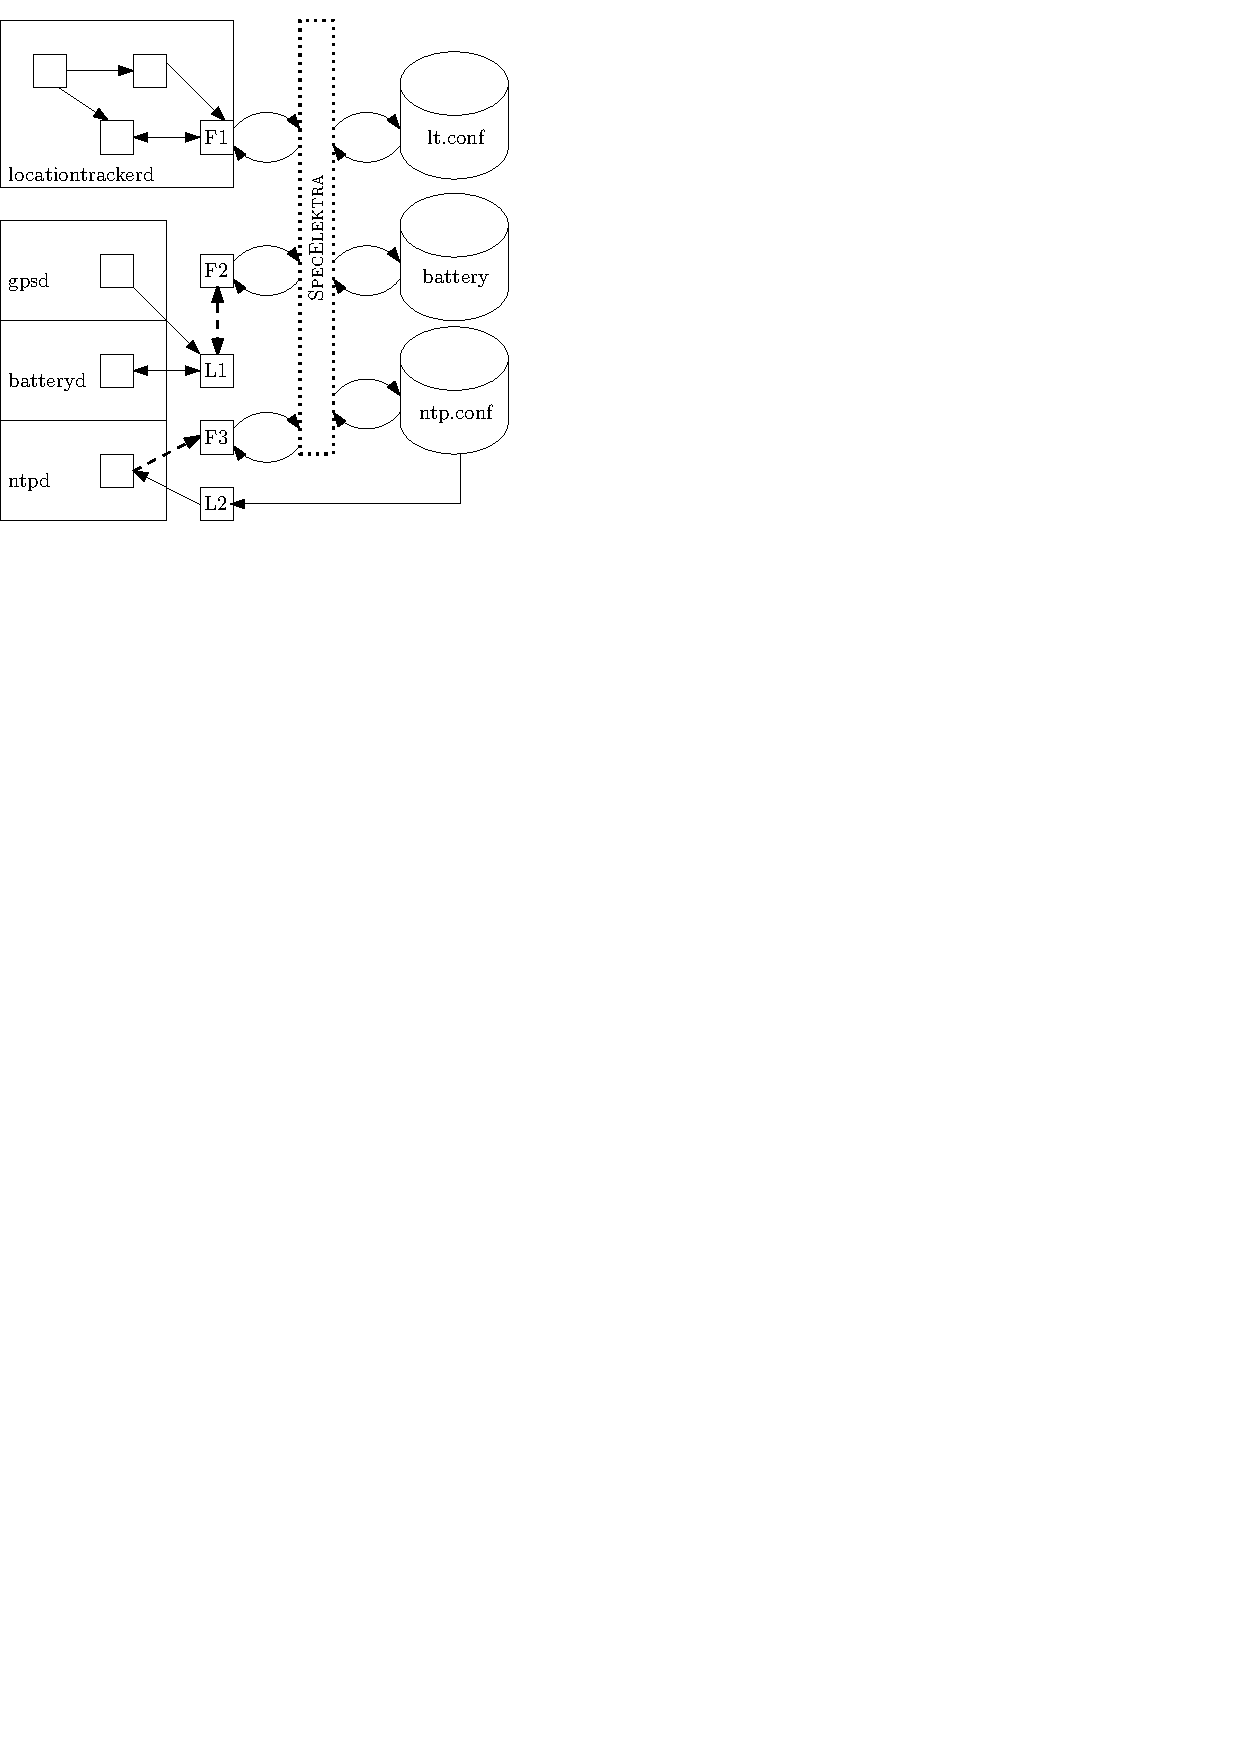
\includegraphics{verticalmodularity}
\caption[Vertical modularity.]{Vertical modularity of locationtracker device. \textnormal{Boxes are applications, cylinders are configuration files, F? are frontends or frontend adapters, L? are configuration libraries~\cite{raab2016improving}.}}
\label{fig:verticalmodularity}
\end{figure}


``\intro[modularity!vertical]{Vertical modularity} is the degree of separation between different applications.''~\cite{raab2016improving}.
If all applications use the same key database with a single backend or a single configuration file, applications would be coupled tightly.
For example, as shown in Figure~\ref{fig:verticalmodularity}, the applications ^gpsd^ and ^batteryd^ both employ the configuration library ^L1^.
Here we cannot deploy ^gpsd^ nor ^batteryd^ without ^L1^.
We prefer high vertical modularity:
We want applications to stay independent of each other.
If coupling between applications is low, for example every application uses a different configuration library or a different backend, we have a high degree of vertical modularity~\cite{raab2016improving}.

\elektra{} provides two mechanisms to retain vertical modularity:

\begin{itemize}
\item Mounting configuration files facilitates different applications to use their own backend and their own configuration file.
Furthermore, mounting enables integrating existing configuration files into the key database.
Configuration specifications written in \elektra{Spec} allow different applications to share their configuration files with each other in a controlled way.

\item Having frontends that implement existing \empha[application programming interface (API)]{application programming interfaces (API)} decouple applications from each other.
These applications continue to use their specific configuration accesses, but \elektra{} redirects their configuration accesses to the shared key database.
Because of the underlying shared key database these frontends improve on the configuration integration problem.
\end{itemize}


\subsubsection{Mechanism 1: Mounting}

\empha[mounting]{Mounting} allows applications to directly access the configurations settings in configuration files of other applications.
The coupling happens in a controlled way within the configuration specification.
We avoid coupling from applications to configuration files.
We use the following specification to define a mountpoint~\cite{raab2016improving}:

\begin{code}
[ntp]
  mountpoint:=ntp.conf
\end{code}

The property ^mountpoint^ (line~2) specifies the configuration file ^ntp.conf^ to be mounted at ^/ntp^ influencing the subtree with the root ^/ntp^.
In \figref{verticalmodularity} the application ^ntpd^ accesses its configuration file ^ntp.conf^ using the library ^L2^, bypassing \elektra{Spec}.
This application is strongly coupled with ^ntp.conf^.
The same configuration file, however, is also accessible through the mountpoint within \elektra{Spec}, which provides a more modular configuration access~\cite{raab2016improving}.

If the configuration specification does not refer to any configuration settings outside of ^/ntp^, only the configuration file ^ntp.conf^ will be loaded.
Thus, from the view of system calls, we retain the same situation as if the applications would directly parse the configuration file ^ntp.conf^.
For performance-wise decoupling, we rely on the capabilities of the file system.

The reason for the improvement in modularity is that mounting avoids coupling from applications to specific backends or to specific configuration files.
Applications using configuration settings below ^/ntp^ (possibly also indirectly via transformations and links) retain their independence from the concrete configuration file ^ntp.conf^.


\subsubsection{Mechanism 2: Frontends}

Providing different frontends decouples implementation internals of different applications.
In the spirit of the adapter design pattern~\cite{gamma1994design} such frontends implement the need of the application.
In the case of ^F1^ in \figref{verticalmodularity}, the frontend is part of ^locationtrackerd^, providing a better modularity of the system.
\elektra{} eases creating new frontends by providing access to configuration settings via lookups in the key set.
Frontends only need to access and update the key set and call ^kdb.get^ and ^kdb.set^ accordingly.

Such frontends are used without any knowledge and concession of applications.
For example, ^L1^ tries to open a configuration file with the system call ^open^.
Because ^F2^ intercepts this system call (dashed line), ^L1^ uses \elektra{} instead.
Then the library ^L1^ parses a configuration file dynamically serialized by \elektra{Lib}~\cite{raab2017introducing}.
Therefore indirectly, ^gpsd^ and ^batteryd^ participate in \elektra{Spec}.
Modern operating systems provide ways to intercept library and system calls without modifications in the source code.
Neither ^gpsd^, ^batteryd^ nor ^L1^ need any coupling to a configuration library in the source code~\cite{raab2016improving}.

The power of such frontends is not limited to system calls:
We extend it to library invocations, for example ^getenv^.
In Figure~\ref{fig:verticalmodularity}, ^F3^ implements the ^getenv^ interface.
Whenever ^ntpd^ calls ^getenv^, ^F3^ redirects the invocation and requests configuration settings from \elektra{} instead.
Again, even though ^ntpd^ has no source code modifications, ^F3^ makes ^ntpd^ participating in a unified configuration system.

\begin{finding}
Due to the use of application-specific frontends and backends, \elektra{} does not endanger vertical modularity.
\end{finding}

Because the key set allows us to support many frontends, we do not have the necessity to have a single API fulfilling all needs, supporting the requirement:
\reqMinimal*



\subsection{Horizontal Modularity}
\label{sec:backend-horizontal-modularity}

\begin{figure}[htp]
\centering
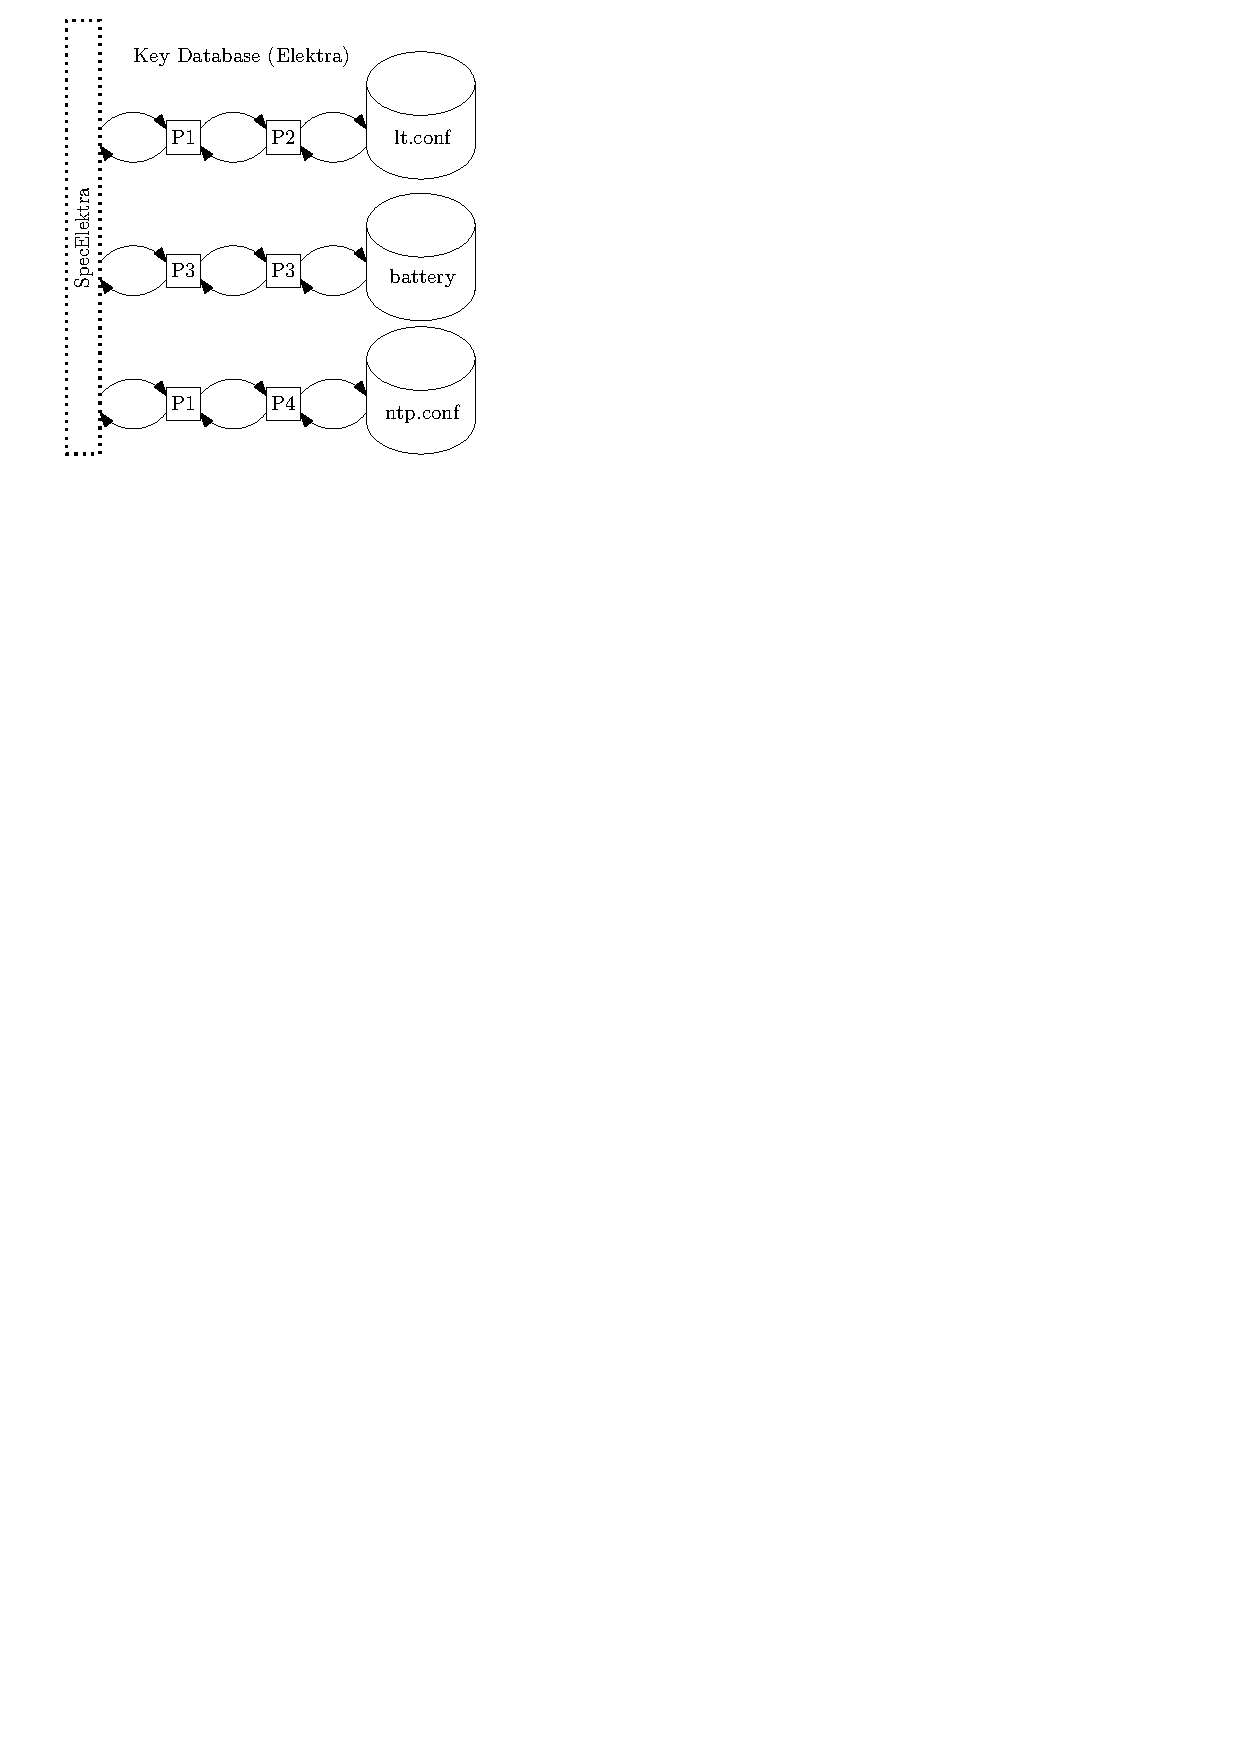
\includegraphics{horizontalmodularity}
\caption[Horizontal modularity.]{Horizontal modularity of locationtracker device. \textnormal{Cylinders are configuration files, P? are plugins~\cite{raab2016improving}.}}
\label{fig:horizontalmodularity}
\end{figure}


In earlier work we defined \intro[modularity!horizontal]{horizontal modularity} to be ``the degree of separation in configuration access code''~\cite{raab2016improving}. 
A higher degree of horizontal modularity allows us to better separate configuration access code and plug the code together as needed.
\elektra{Spec} employs the pipes-and-filters architectural pattern (see ^P1^--^P4^ in Figure~\ref{fig:horizontalmodularity}).
\empha[plugin]{Plugins} are pieces of configuration access code that share the same interface.
Three factors of \elektra{Spec} improve horizontal modularity:

\begin{enumerate}
\item
Using \elektra{Spec}, applications are completely decoupled from configuration specifications.

\item
The plugin assembling algorithm described in \secref{plugin-assembly} abstracts the specifications written in \elektra{Spec} over concrete plugins.
\elektra{} has no dependence to other libraries but only concrete plugins introduce dependences.
We achieve a system-level dependence injection.

\item
The \empha{provider} abstractions in the dependences between the plugins abstract over concrete implementations of configuration access code.
Here we reduce the coupling between plugins.
\end{enumerate}

\begin{finding}
Moving configuration specifications and dependences from the applications' source code to configuration specifications and plugins improves horizontal modularity.
\end{finding}

We improve on Requirement~\reqref{dependences}:
\reqDependences*




\subsubsection{Generic Plugins}


Here we describe a technique how we facilitate a single implementation of a plugin to create different plugins with different features sets.
By making plugins more fine-granular, we achieve better horizontal modularity.


We say a plugin is \intro[plugin!generic]{generic} if its feature set cannot be described in a single contract.
We distinguish between static and dynamic generic plugins.
Dynamic generic plugins have non-trivial plugin configuration such as behavioral descriptions, programs, or scripts.
For example, the script plugin \plugin{lua} is a dynamic generic plugin.
The plugin configuration ^script^ specifies a Lua-script~\cite{raab2016improving}:



\begin{code}
[locationtrackerd]
  infos/plugins:=lua script=batterytotracker.lua
\end{code}

Different scripts cause the dynamic generic plugins to require different contracts.
We need to take care about not confusing such plugins:
They have the same plugin name but otherwise are hardly related~\cite{raab2016improving}.


The static type of generic plugins facilitates compile-time conditionals, which we call \intro[compilation variant]{compilation variants}.
They can only be used if the plugin is written in a programming language that supports compile-time decisions, for example, macros in C.
Here the compiler resolves variability.
Compilation variants are beneficial if~\cite{raab2016improving}:

\begin{enumerate}
\item We need performance, which conflicts with flexibility.
\item We need the plugin during \empha{bootstrapping}, where we cannot provide plugin configuration \cite{raab2015kps}.
\item We need nearly-identical plugins depending on different APIs, which cannot coexist in the same plugin.
\end{enumerate}

We compile the plugin's code with requested combinations of defined and undefined macros.
Different combinations of macros then can yield different contracts.
For example, the plugin \plugin{crypto} decides which cryptography library should be used via compilation variants~\cite{raab2016improving}.%
{\parfillskip=0pt plus .8\textwidth \emergencystretch=.6\textwidth \par}

\subsection{Suitable Configuration Settings}
\label{sec:backend-suitable}

We propose to use configuration settings to encode requirements.
Other configuration settings derive information from these configuration settings.
We aim at \empha[suitable configuration]{suitable} context-aware configuration.

\begin{example}
A software running on different devices with different requirements would use the following specification as requirement~\cite{raab2016improving}:

\begin{code}[morekeywords={enum,0,1,2}]
[device]
  check/enum/#0:=wearable
  check/enum/#1:=smartphone
  check/enum/#2:=car
\end{code}

The configuration setting ^device^ can have three different configuration values: wearable, smartphone, or car.
\end{example}

To map the configuration settings encoding information for requirements to concrete configuration settings, configuration value transformations are needed.
The most important transformation is assignment between configuration settings:

\begin{example}
As discussed in~\cite{raab2016improving}:

\begin{code}[morekeywords={assign}]
[powersaving/gps]
  assign/condition:=(device != 'car') ? (battery/level) : ('0')
[gps/resolution]
  assign/condition:=(device == 'car') ? ('high') : ('low')
\end{code}

We facilitate the plugin \plugin{conditionals} that allows us to specify conditions with two branches.
\elektra{Spec} ensures that the keys \key{powersaving/gps} and \key{gps/resolution} are always set according the requirements defined in ^device^~\cite{raab2016improving}.
\end{example}

We are not limited to transformations from configuration settings encoding requirements.

\begin{example}
We want a device with a low battery to stop polling GPS.
Again we use conditionals~\cite{raab2016improving}:


\begin{code}[morekeywords={assign}]
[gps/status]
  assign/condition:=(battery/level > 'low') ?  ('on') : ('off')
\end{code}
\phantom{}
\end{example}


\subsection{Modular Type Checking}
\label{sec:backend-type}

Compared to checking of configuration specifications, type checking of configuration settings has a more direct impact on the system.
If the validation is not rigorous enough, misconfiguration is not caught.
A too complicated specification language, however, would be avoided by developers.
No further dependences shall be added to the application if new validation specifications are added:
\reqDependences*

To fulfill these diverse requirements, \elektra{} does not have a single way to validate configuration.
Instead \elektra{} provides a \empha{modular configuration specification language} that enables developers to create their own validation languages.
One rationale is that \elektra{} validates configuration values to be consistent with their context, even if the context is not encoded as configuration setting.
Here we might need language constructs for every kind of context.
For example, users not only need validations whether a configuration setting contains an IP address but they also need validations whether the address points to a reachable service.
We got the following feedback during the survey described in \chapref{motivation}:
\emph{``There are variables which have a huge list of possible values. These lists are taken from databases. So at the end we have two sources for the possible values: the configuration specification and the database''}.

We could integrate file system metadata, the surrounding network topology, and other databases within the key database.
Then we would exclusively validate data without external factors.
Integrating all data in \elektra{} crosses the border of having a tool that is specific enough to be useful.
Integrating huge databases, as requested in the survey, conflicts with other requirements of \elektra{}.

We propose to have a modular configuration specification language in which users add their own configuration specification constructs and implement them as plugins.
Users shall be able to combine already existing validation plugins with their own validation plugins.
For example, a user writes a validation plugin querying large databases.

\subsubsection{Pluggable Type System}

We extend on the ideas of pluggable type systems~\cite{andreae2006framework,haldiman2009practical,papi2008practical}.
The idea of pluggable type systems is to guarantee the absence of additional errors that would not be detected by the built-in type system.
Users \emph{``should be able to choose the kind of static checks one would like to perform''}~\cite{haldiman2009practical}.
This way, we do not introduce problems if we add an exotic type system for a single application.

For \elektra{Spec}, we decided to adapt such a flexible approach and users can plug in arbitrary type checkers.
\citet{papi2008practical} suggested to use annotations for additional type information.
Based on the idea, we use properties of keys to describe data types:

\begin{code}[morekeywords={restrict,null,write,enum,path}]
[slapd/threads/listener]
  check/type:=long
  check/range:=1,2,4,8,16
\end{code}

In line~2, the property \property{check/type} states that we use the CORBA data type ^long^.
Different to specifications with the property \property{type}, we use the data type only for validation and not for code generation.
In line~3 we further restrict the configuration setting to some specific values.
Because line~3 specifies the configuration setting in a stricter way, line~2 does not have an influence on the configuration validation.
\elektra{Spec}'s syntax is verbose but with the advantage that adding extensions never causes conflicts because our model requires us to always use fresh property names.

\subsubsection{Two-phase Checking}


To provide maximum flexibility and modularity, the checking of the structure and data types is separated.
This separation establishes a \intro[two-phase type checking]{two-phase type checking}:


\paragraph{Checking structure:}
For some applications, missing keys is as fatal as non-validated keys.
In a first phase, the structure of the specification is enforced.
The phase makes sure that keys (not) allowed to occur are (not) present.
Additionally, it applies concrete dynamic type information as properties to keys by matching key names with \empha{glob} expressions.
\begin{example}
The plugin \plugin{spec} is a plugin that checks structure and supports following glob expressions:
\begin{description}
\item{\texttt{\_}} denotes an arbitrary hierarchy level, and
\item{\texttt{\#}} denotes an arbitrary array index.
\end{description}
Thus the specification ^[a/_/key/#]^ will match keys such as:

\begin{code}[language=CfgElektra]
a/simple/key/#0=
a/nother/key/#_12=value not part of match
\end{code}

The plugin \plugin{spec} also copies metadata to every matching configuration setting.
\end{example}

\paragraph{Checking values:}
In a second phase, the checks given by metadata copied in the first step are checked for each key.
These two phases are independent of each other and have their own use cases.
For the second phase, many data types are supported.

\subsubsection{Data Types}
\label{sec:data-types}

We already introduced \property{check/type} and \property{check/enum} which are two of the data types.
\elektra{} supports many other data types, each implemented in its own plugin(s):
\begin{description}
\item [check/type] allows us to specify CORBA data types, as already listed in \exref{types} on page \pageref{ex:types}.
Checking ^any^ is always successful.
The record and enum types defined by CORBA are not part of this plugin but of others as explained below.

\item [check/enum] supports a list of supported values denoted by array indexes.
\item [check/bool] transforms specific strings, for example ^true^ and ^false^, into the canonical boolean representation, i.\,e., ^0^ and ^1^.
\item [check/ipaddr] checks if a string is a valid IP address.
\item [check/path] checks presence, permissions, and type of paths in the file system.
\item [check/date] supports to check date formats such as POSIX, ISO8601, and RFC2822.
\item [check/validation] checks the configuration value with regular expressions.
\item [check/condition] checks using conditionals and comparisons.
\item [check/math] checks using mathematical expressions.
\item [check/range] allows us to check if numerical values are within a range.
\item [trigger/error] allows us to express unconditional failures.
\end{description}

\elektra{} supports binary and string types.
Binary configuration values can include null characters in their string and can have the special value $\NullValue$.
Because binary is only used on special occasions, for example to represent encrypted values, all validations are only against string types.

The data types form a lattice, with ^error^ as bottom and ^any^ as top element~\cite{harkes2016icedust,haldiman2009practical}.
By default, every key has the type ^any^ regardless if it is specified using ^[]^ or not.
Adding specifications without any properties is useful:
It tells the user which of the configuration settings are relevant for an application.
Every property that additionally specifies a type restricts the range of allowed values.

\subsubsection{Discussion}

Up to now, we used type restrictions, also known as \intro{subtype} in Ada.
In \elektra{} the specifications are even more flexible than in Ada:
They allow a type to be a list of any checkers.
Each of these checkers make the type stricter.
This fact makes the types in \elektra{} safe to use, even though \elektra{}'s types do not have a closed model (and thus can be neither sound nor complete).
The trouble-free combination of many checkers is a pragmatic decision.


To define a structured type, we use the ideas of Relax~NG~\cite{clark2002relax}.
Our language, defined by the plugin \plugin{spec}, is simpler because neither attributes nor XML namespaces exist.
Instead of repeating key names, we make key names unique by adding array indexes.
A specification without any property, for example ^[x]^, is equivalent to Relax~NG's ^zeroOrMore^ which is the same as Relax~NG's ^optional^ in our case.
In the area of structured types, the lack of a closed model is problematic as features can have unnecessary overlap.
The advantage of our open model is that every developer can participate and applications can choose to use completely different models for their validation specifications.
















































\section{Context awareness without Source-code Modifications}
\label{sec:unmodified-floss}

Instead of improving configuration access APIs as done in the previous \chapref{frontend}, in this section we focus on providing the best user experience with existing configuration access APIs.
The idea is to facilitate \empha[configuration access point]{configuration access points} present in applications.
We retrofit legacy applications by combing the already introduced:%
{\parfillskip=0pt \emergencystretch=.5\textwidth \par} %needed to align applications.
\begin{itemize}
\item context-aware lookup from~\secref{backend-context-aware-lookup} (as specified in \secref{approach-context-aware-lookup}), and
\item modularity and adaptation of frontends from~\secref{modular-abstractions}.
\end{itemize}
Such a functionality is important because rewriting all applications to new configuration access APIs is unrealistic.
Legacy applications will always play an important role:
What we implement today, will be legacy tomorrow.
We want to improve on the requirement:%
{\parfillskip=0pt \emergencystretch=.6\textwidth \par}
\reqLegacy*

We focus on free and open source software (FLOSS) and configuration access APIs usually present there.
We claim that it is feasible and practical to use software without source code modifications, and by run-time reconfiguration, upgrade their context awareness.
We aim at exploiting already existing configuration access points in free and open source software~\cite{raab2017introducing}, answering:
\rqBackendContextUnmodified*

\subsection{Demand}

As already stated, context awareness is not an absolute measure.
Instead \empha[viewpoint]{viewpoints} always create demand for more context awareness.
We usually do not learn about such situations before we discuss them with a user.
These conflicts with current ideas of \empha[context-oriented software engineering]{context-oriented software engineering} where context needs to be considered already at design time~\cite{kamina2014context}.
Hence, context-oriented software engineering is not applicable to existing large software projects where context is not known beforehand, neither for legacy software~\cite{raab2017introducing}.

To improve on this problem, we propose to delay context-oriented software engineering to deployment-time.
This way we move decisions about supported contexts to a time when more about the required contexts is known.
We classified three \empha[stakeholder]{stakeholders}~\cite{raab2017introducing}:%
{\parfillskip=0pt \emergencystretch=.7\textwidth \par}
\begin{itemize}
\item the developers, who implement programs with variations useful for context awareness, without defining which variation is used in which situations,
\item the system administrators, who enable context awareness in their systems with our novel context-oriented software engineering during deployment, and
\item the end users, who enjoy better context awareness in their systems and can report missing context awareness to system administrators.
\end{itemize}

As running example in this section, we use mobile workplaces.
For browsers the network connection is an important context.
With different network connections, we require different proxy settings.
We aim at browsers automatically adapting themselves to the current context.
We want browsers to be aware of the current network connection, of the nearest printers, etc.~\cite{raab2016unanticipated}.



\subsection{Configuration Access APIs}

To avoid any source code modifications, applications must fulfill the following assumptions to be suitable for \elektra{}:
\begin{enumerate}
\item The applications must have configuration access points present in the source code.
\item Without extensions, we require the use of configuration access APIs at configuration access points.
For example, configuration access points that access data structures and variables are currently not supported.
We do not impose restrictions on the gestalt of the configuration access APIs.
\item For flawless context awareness the configuration access points must be triggered perpetually;
and not only once at start-up.
\end{enumerate}

Assumption~3 is not strictly necessary, but without it, dynamic adaptation is not possible.
Instead we would need to restart applications on context changes.
We focus on situations where such restarts are not necessary.

Based on our earlier studies in \chapref{motivation} these assumptions are reasonable.
Applications have plenty of configuration access points, often in the form of an API, which are called repeatedly.
We did not show, however, whether configuration access points control behavior that is of interest for context awareness.

\subsubsection{\texttt{getenv}}

The ^getenv^ API\index{getenv|boldindex} enables developers to query environment variables.
\intro[environment variable]{Environment variables} live in a data structure called ^environ^ within the processes.
They are initialized once at program startup.
In the current implementations, only the process itself can update ^environ^.

If the user changes an environment variable, for example ^PATH^, only new subprocesses see the change.
This can be wanted, for example, if choosing which compiler to be used for the next compilation process.
Most often, however, this is unwanted and a major usability problem.
For example, a user modifying ^http_proxy^ needs to logout and restart all relevant daemons.

We include ^getenv^ for our investigations because it~\cite{raab2017introducing}
\begin{itemize}
\item is widely standardized, including SVr4, POSIX.1-2001, 4.3BSD, C89, C99~\cite{man2017getenv},
\item and is supported by many programming languages.
\end{itemize}

\subsubsection{\texttt{open}}

Applications use the ^open^ API\index{open|boldindex} to open configuration files.
Its return value is a file handle, which is processed by further system calls.
Usually, applications use it indirectly via some higher-level API, such as ^fopen^.
Different from ^getenv^, the file system is designed for inter-process communication.
Hence, applications can implement reloading of configuration settings on configuration file changes.

The ^open^ system call is
\begin{itemize}
\item standardized by SVr4, 4.3BSD, POSIX.1-2001, POSIX.1-2008~\cite{man2017open},
\item and available in every relevant programming language, although sometimes with restrictions for security reasons.
\end{itemize}





\subsection{Approach}

To make applications use \elektra{} without any source code modifications, we hijack their API calls.
For example, Web browsers contain code such as~\cite{raab2017introducing}:

\begin{code}
getenv ("http_proxy");
\end{code}

Conventional implementations of ^getenv^ would return an outdated proxy after network changes because environment variables cannot be corrected from outside of processes.
We interpret such ^getenv^ accesses as reading a contextual value~\cite{raab2017introducing}.
Replacing the ^getenv^ implementation with \elektra{}'s context-aware lookup, unmodified applications will use context-aware configuration.
Contrary to standard ^getenv^, the configuration setting are consistent with the content of configuration files, fulfilling the requirement:
\reqConsistency*


\subsubsection{Interception}

\elektra{} with interception works as follows:
\begin{itemize}
\item We intercept a pre-^main^ method.
In it \elektra{} \empha[bootstrapping]{bootstraps} itself with the help of initial configuration files.
The initial configuration files contain both the configuration settings and specifications for the contextual values~\cite{raab2017introducing}.
At this early stage we will pass command-line options to \elektra{}.
\item If the application calls ^open^ with its configuration file as argument,
\elektra{} serializes a configuration file on-the-fly and returns a file handle to it.
\item If the application calls ^getenv^ with a parameter specified in \elektra{Spec},
\elektra{}'s context-aware lookup is invoked.
\end{itemize}

Unfortunately, interceptions of library invocations are platform-dependent.
But every major operating system provides some techniques for interceptions.
We implemented the interception techniques for GNU/Linux using ^LD_PRELOAD^ and ^/etc/ld.so.^\linebreak^preload^~\cite{raab2017introducing}:%
{\parfillskip=0pt plus .8\textwidth \emergencystretch=.5\textwidth \par}
\begin{itemize}
\item
The environment variable ^LD_PRELOAD^ allows us to preload libraries.
Then the symbols of the preloaded library are preferred.
This technique does not work during boot-up of the system.
\item
The configuration file ^/etc/ld.so.preload^ has the same purpose but does not have ^LD_PRELOAD^'s restriction.
Libraries mentioned in this file are automatically preloaded for every process.
We prefer this method, and registered our library, which implements ^getenv^ and ^open^, in this configuration file.
\end{itemize}



\subsubsection{Context Specification}

In \elektra{Spec}, the user has to define which ^getenv^ parameters and configuration files shall be controlled by \elektra{}.
In our approach, the frontend responsible for the interception reads the layers and configuration specifications from keys below ^/env^:
\begin{description}[font=\texttt]
\item[/env/layer] contains the layers to use.
\item[/env/override] contains the keys that shall be preferred to environment variables.
\end{description}


\begin{example}
Let us specify the return value of ^getenv("http_proxy")^~\cite{raab2017introducing}:

\begin{code}
[env/override/http_proxy]
  context:=/http_proxy/%interface%/%network%
\end{code}

Then \elektra{} takes control over every ^getenv^ invocation that has the parameter ^http_proxy^.
Line~2 is the specification as defined in \secref{approach-context-aware-lookup}.
The context-aware lookup ensures that the contextual value recursively considers context specifications.
After layer switches, the same requested key name can yield different values.
We use a configuration file containing the mapping to concrete values~\cite{raab2017introducing}:

\begin{code}[language=CfgElektra]
http_proxy/wlan/home=proxy.example.org
http_proxy/eth/work=proxy.example.com
http_proxy/%/%=default.example.com
\end{code}

If ^interface^ changes to ^eth^ and the ^network^ to ^work^, the next invocation of ^getenv("http_proxy")^ returns ^proxy.example.com^~\cite{raab2017introducing}.
\end{example}

\subsubsection{Context Changes}
\label{sec:context-changes}

To always reflect external changes of the context, we have two options.
We either pull changes, or a \empha{context sensor}, as introduced in \secref{context-sensors}, pushes changes to all applications.
We implemented both approaches to support more applications and APIs.

Pulling changes works well for configuration access APIs that are called repetitively, such as ^getenv^.
\elektra{}'s ^getenv^ implementation uses the following algorithm~\cite{raab2016unanticipated}:%
{\parfillskip=0pt \emergencystretch=.5\textwidth \par}

\begin{code}[language=Cpp,escapeinside={(*@}{@*)}]
KeySet conf; // global variable used by reload* functions
char * getenv (const char * key)
{
	if (reloadNeeded ())
	{
		reloadConfiguration ();
		reloadLayers ();
	}
	return ksLookup (conf, Key ("/env/override/" (*@$\concat$@*) key));
}
\end{code}

The continuous polling makes sure that every ^getenv^ considers the latest layers and configuration settings.

For other configuration access APIs polling does not work.
For example, most applications call ^open^ already at startup but provide a way to trigger reinitialization.
In such situations, we use a plugin that triggers application on configuration changes.


\begin{figure}[htp]
\centering
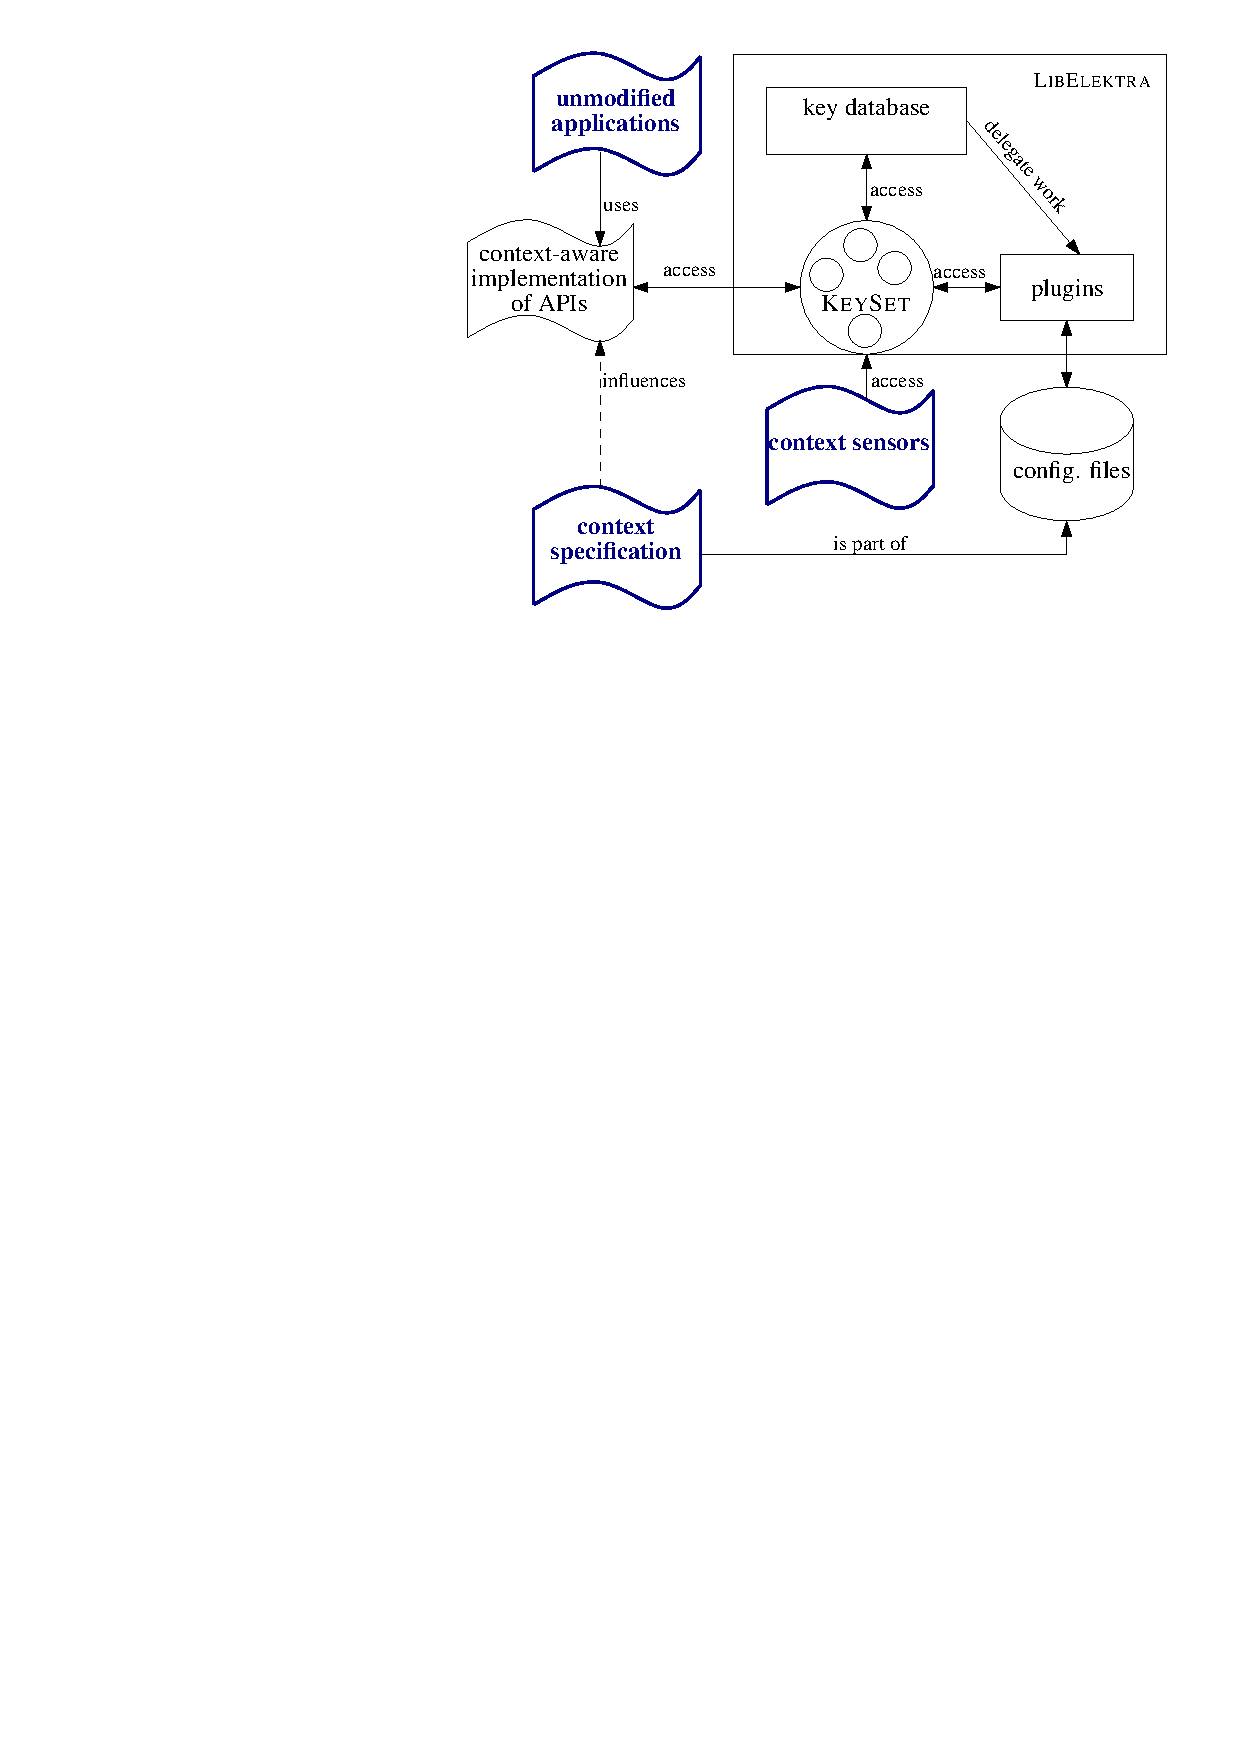
\includegraphics{getenvarchitecture}
\caption[Architecture of \elektra{} with interception.]{Architecture of \elektra{} if used with interception.
The common data structure is the key set (shown in the middle).
Bold, blue boxes need to be provided by the users of \elektra{}~\cite{raab2016unanticipated}.}
\label{fig:getenvarchitecture}
\end{figure}

This architecture shown in \figref{getenvarchitecture} ensures complete decoupling between context sensors and applications.
Thus the same context sensors are reused for many applications.

In the running example, users change their location or connect a network cable.
A context sensor recognizes such changes and modifies the key database accordingly.
The key database executes the plugins that trigger the applications to reparse their configuration files when using ^open^ interception.
For ^getenv^ interceptions the triggering is not necessary because of the polling.



\subsection{Context-oriented Software Engineering Process}
\label{sec:cose-process}

Here we describe a process of how our approach is applied.
We expand on our running example, and show how to use \elektra{} to enable flexible workplaces.
The requirements were that applications such as Firefox shall automatically use (1) the nearest printer, and (2) the correct proxy.

\begin{figure}[htp]
\centering
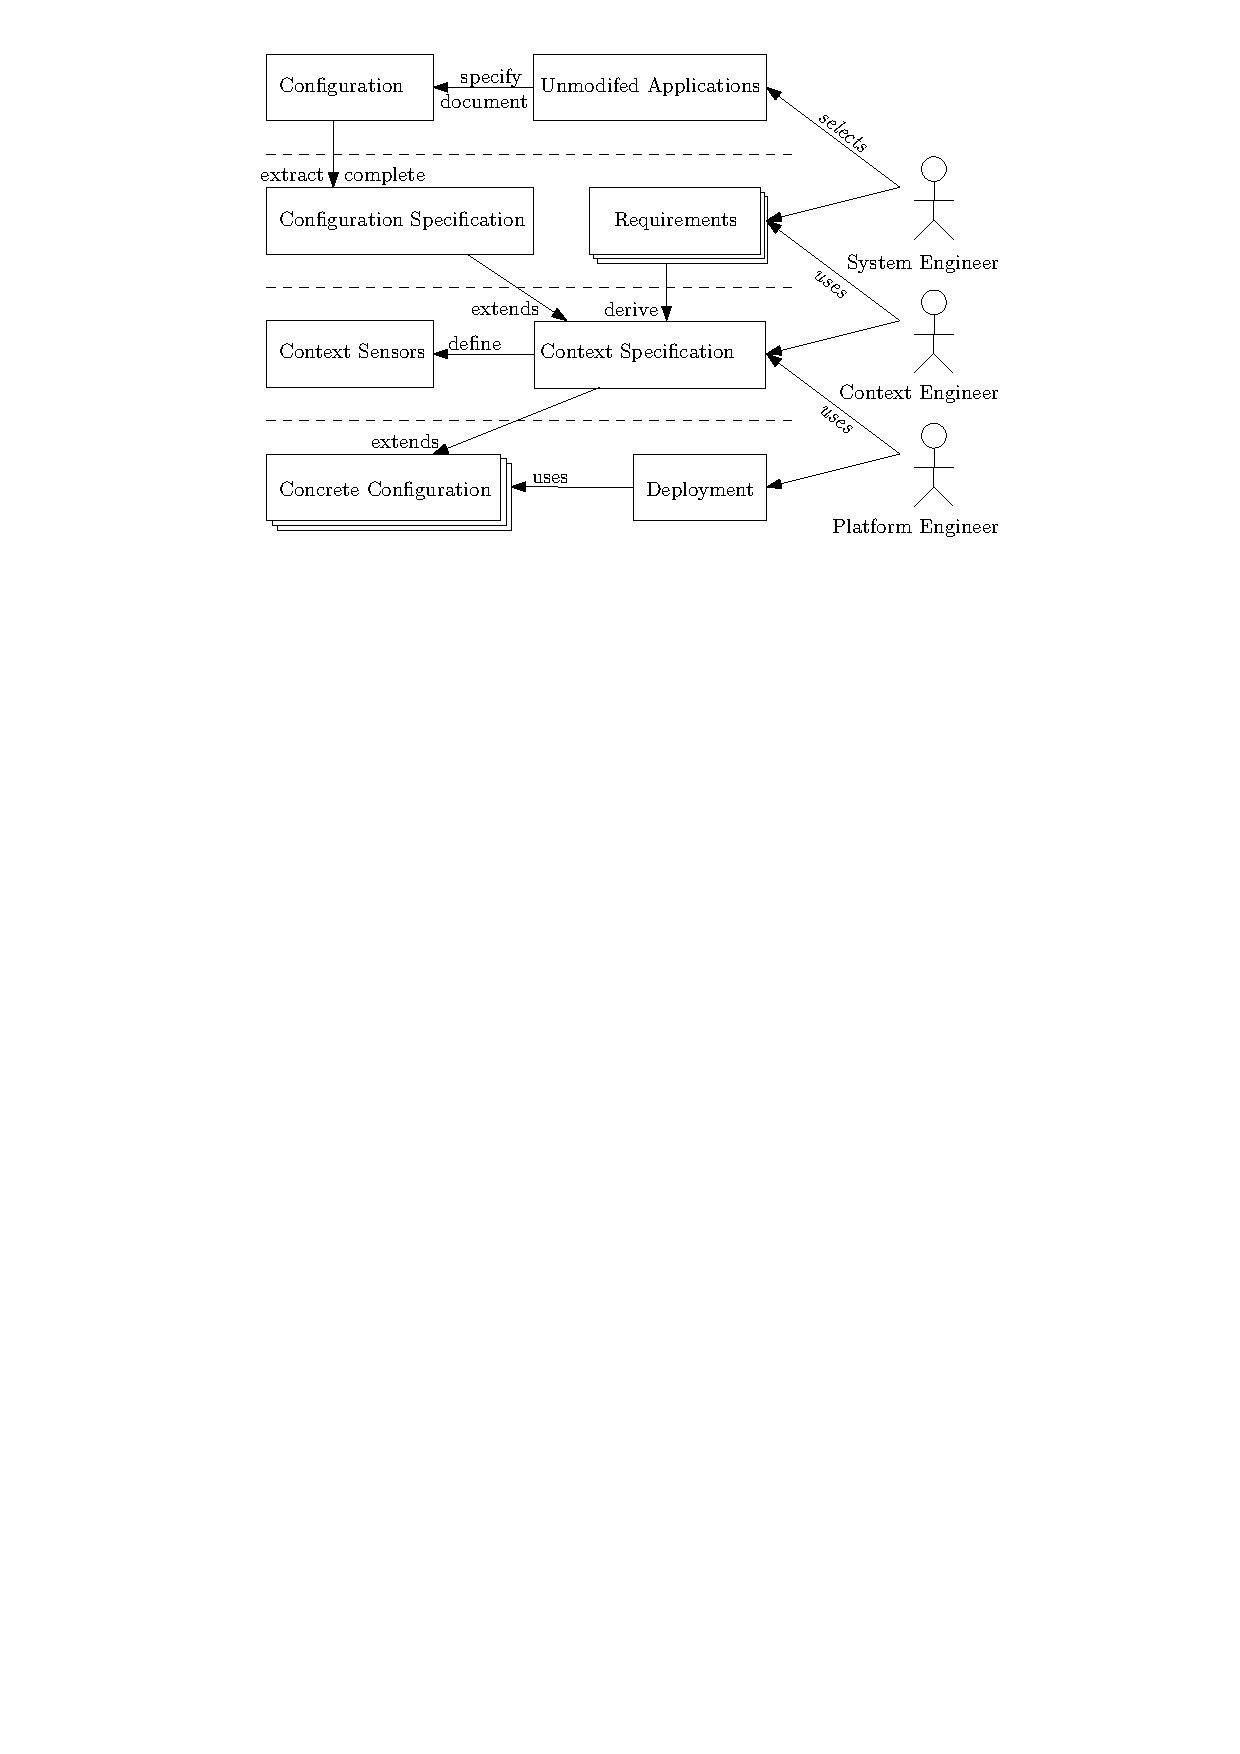
\includegraphics{process}
\caption{Context-oriented software engineering process.}
\label{fig:process}
\end{figure}

As shown in Figure~\ref{fig:process} we split up the engineering team into the roles of system, context, and platform engineers.
In large organizations these roles are implemented by different teams.
Otherwise, different persons act according to the role they get assigned.

System engineers first define the requirements.
Then they decide which applications shall be used.
They document their decisions and complete the specification of relevant configuration settings.

In our running example, one of our requirements is that the browser picks up proxy settings automatically.
Then the system engineers investigate if Firefox has all needed settings and find it is enough to intercept ^getenv^.
They choose Firefox as the unmodified application to use.

In the role of context engineers we extracted relevant contexts from the previously constructed requirements.
Context-oriented software engineering works with the hypothesis that \emph{``The factors dynamically changing the system behavior are candidates for contexts''}~\cite{kamina2014context}.
They consider ``changing of workplace'' as context.
Based on the context, engineers specify the layers.
We decided the relevant context consists of two layers:
The layer ^network^ differs for every workplace.
The layer ^interface^ distinguishes how someone is connected to the workplace's network.
This permits a user in the same location, but connected via a wireless network, to see different printers and use a different proxy as someone connected via cable.
We specified ^http_proxy^ and ^PRINTER_LIST^ to automatically use the nearest printer:

\begin{code}
[env/override/http_proxy]
  context:=/http_proxy/%interface%/%network%
[env/override/PRINTER_LIST]
  context:=/printer/%interface%/%network%
\end{code}

The context engineers then implement a context sensor that updates the layers ^interface^ and ^network^.
The context engineers adapt their network scripts such that the layers are always set according to the workplace in use.
In the example, the context sensors are trivial one-line hooks in the ^/etc/NetworkManager^ scripts.

In the last step, the platform engineers deploy the applications on the organization's platforms.
They enrich the configuration settings with platform-specific configuration settings such as concrete proxies and printers.
Finally, they install the artifacts and configuration files produced in the previous steps.


